				
\section{Results}

\subsection{Getting Started with Bonsai}

\subsubsection{Community}

The Bonsai framework can be downloaded at \url{https://bitbucket.org/horizongir/bonsai} and installed on Windows operating systems starting with Windows 7 and above. The website is organized into different sections: Downloads (where the latest installer is located), Wiki (with a “Getting Started” guide, tutorials and (FAQ) frequently asked questions), and Issues (where bugs can be reported). We have also created a user forum (address is listed in the FAQ section) where the community of Bonsai users have been sharing their feedback, questions and experiences.

A video tutorial introduction to Bonsai is included with this publication (Supplementary Video 1).

\subsubsection{Extending Bonsai}

Bonsai was designed from the outset to support many different layers of extensibility:
\begin{enumerate}[(a)]
    \item Dataflows: The first layer is through the creation of Bonsai dataflow files themselves. Existing dataflows can be directly reused inside other dataflows as nested nodes. This allows for the sharing of reusable dataflow design patterns between applications.
    \item Python Scripting: Bonsai supports embedded scripting using IronPython 2.7. Specifically, Bonsai includes three types of Python nodes: PythonTransform, PythonCondition, and PythonSink, which all operate by calling a user-defined Python function described by a script. Below we include a simple example of a PythonTransform for rescaling data:

    \begin{lstlisting}[language=Python]
# Declare transform output type
@returns(float)
def process(value):
    return value / 255.0
    \end{lstlisting}

    \item NuGet: Bonsai modules are natively written in C\# or other.NET languages. The NuGet package manager has emerged as the defacto standard for the sharing of code between.NET developers. Bonsai includes a full NuGet client which manages local package versions, provides access to the curated feed of standard Bonsai packages, and allows for the quick sharing of modules between Bonsai users through either NuGet or other remote and local package sources. Tutorials and examples on how to create new Bonsai modules are included in the Wiki.
\end{enumerate}

\subsection{Under the Hood}

\subsubsection{Computational Overhead}

Bonsai takes full advantage of the flexibility of C\# and its Just-In-Time (JIT) compiler to bring the computational overhead of running the framework to zero. This is possible due to the fact that the graphical dataflows in Bonsai are actually specifying syntactically correct C\# code by means of an expression tree. When the dataflow is executed, C\# code is generated for assembling and running the pipeline. This code is ultimately compiled into native machine language before execution, which has the consequence that running a Bonsai dataflow is as fast as if one wrote the equivalent Rx code manually. In fact, this also means every Bonsai module is just a standard C\# class exposing methods working on Rx's observable interface, which makes it possible to reference every single Bonsai package from a standard.NET application and just use the module functionality directly.

\subsubsection{Concurrency}

The level of concurrency and parallelism in Bonsai entirely depends on the structure of each individual dataflow and the specific computer hardware involved. Typically, each hardware device source (e.g., a camera) runs independently in its own logical thread. Some sources can occasionally share threads when the underlying device architecture allows for it. For example microcontroller sources coming from the same USB port effectively require sharing a single communications channel, but this is logically abstracted from the developer so there is no need to worry about handling multiplexed messages.

The specialized handling of concurrency introduced by merging different processing streams is done using dedicated Rx concurrency operators that are exposed graphically through the language. Operators located downstream from the merge point can treat the merged sequence as if it was a single sequential data source. This means most Bonsai operators are actually concurrency-agnostic, meaning they don't have to worry about concurrency at all: they simply assume their inputs are processed sequentially. This functional approach allows Bonsai operators to be simple to program, reliable and extremely performant.

Finally, some Bonsai operators introduce local concurrency implicitly to maximize performance. For example, many of the data logging sinks actually write to disk in parallel with the arrival of data. This prevents processor-heavy routines, such as video compression, to stall the pipeline and allow for online execution to proceed as fast as possible. From the point of view of the developer, however, such optimizations happen transparently.

\subsubsection{Time}

Being a fully asynchronous framework, Bonsai has to deal with code executing logically in many different processors. There is no particular assumption about time in the framework other than the sequential flow of data through the pipeline, but facilities are in place to help the synchronization and timing of data. For example, the Timestamp operator provides access to hardware performance timers included in modern processors to timestamp event notifications, across the pipeline, using a shared high resolution clock. However, it should be noted that this only applies to processes occurring centrally: for precise sub-millisecond synchronization of physical events happening outside the computer (e.g., stimulation pulse train and electrophysiology data) we still recommend the classical sharing of voltage or optical sync pulses logged simultaneously in each device.

\subsection{Applications}

The validation of Bonsai was performed by using the framework to implement a number of applications in the domain of neuroscience (Figure \ref{fig:bonsaiApplications}). The breadth of technologies at use in this field demands that modern experiments be able to handle many heterogeneous sources of data. Experimenters need to routinely record video and sensor data monitoring the behaviour of an animal simultaneously with electrophysiology, optical reporters of neural activity or other physiological measures. Online manipulation and visualization of data is a fundamental part of the experiment protocol for many of the reported techniques. In the following, we highlight some of these practical applications of Bonsai in more detail in order to illustrate both “best practices” and implementation strategies.

\begin{figure}
\begin{center}
\scalebox{0.87}{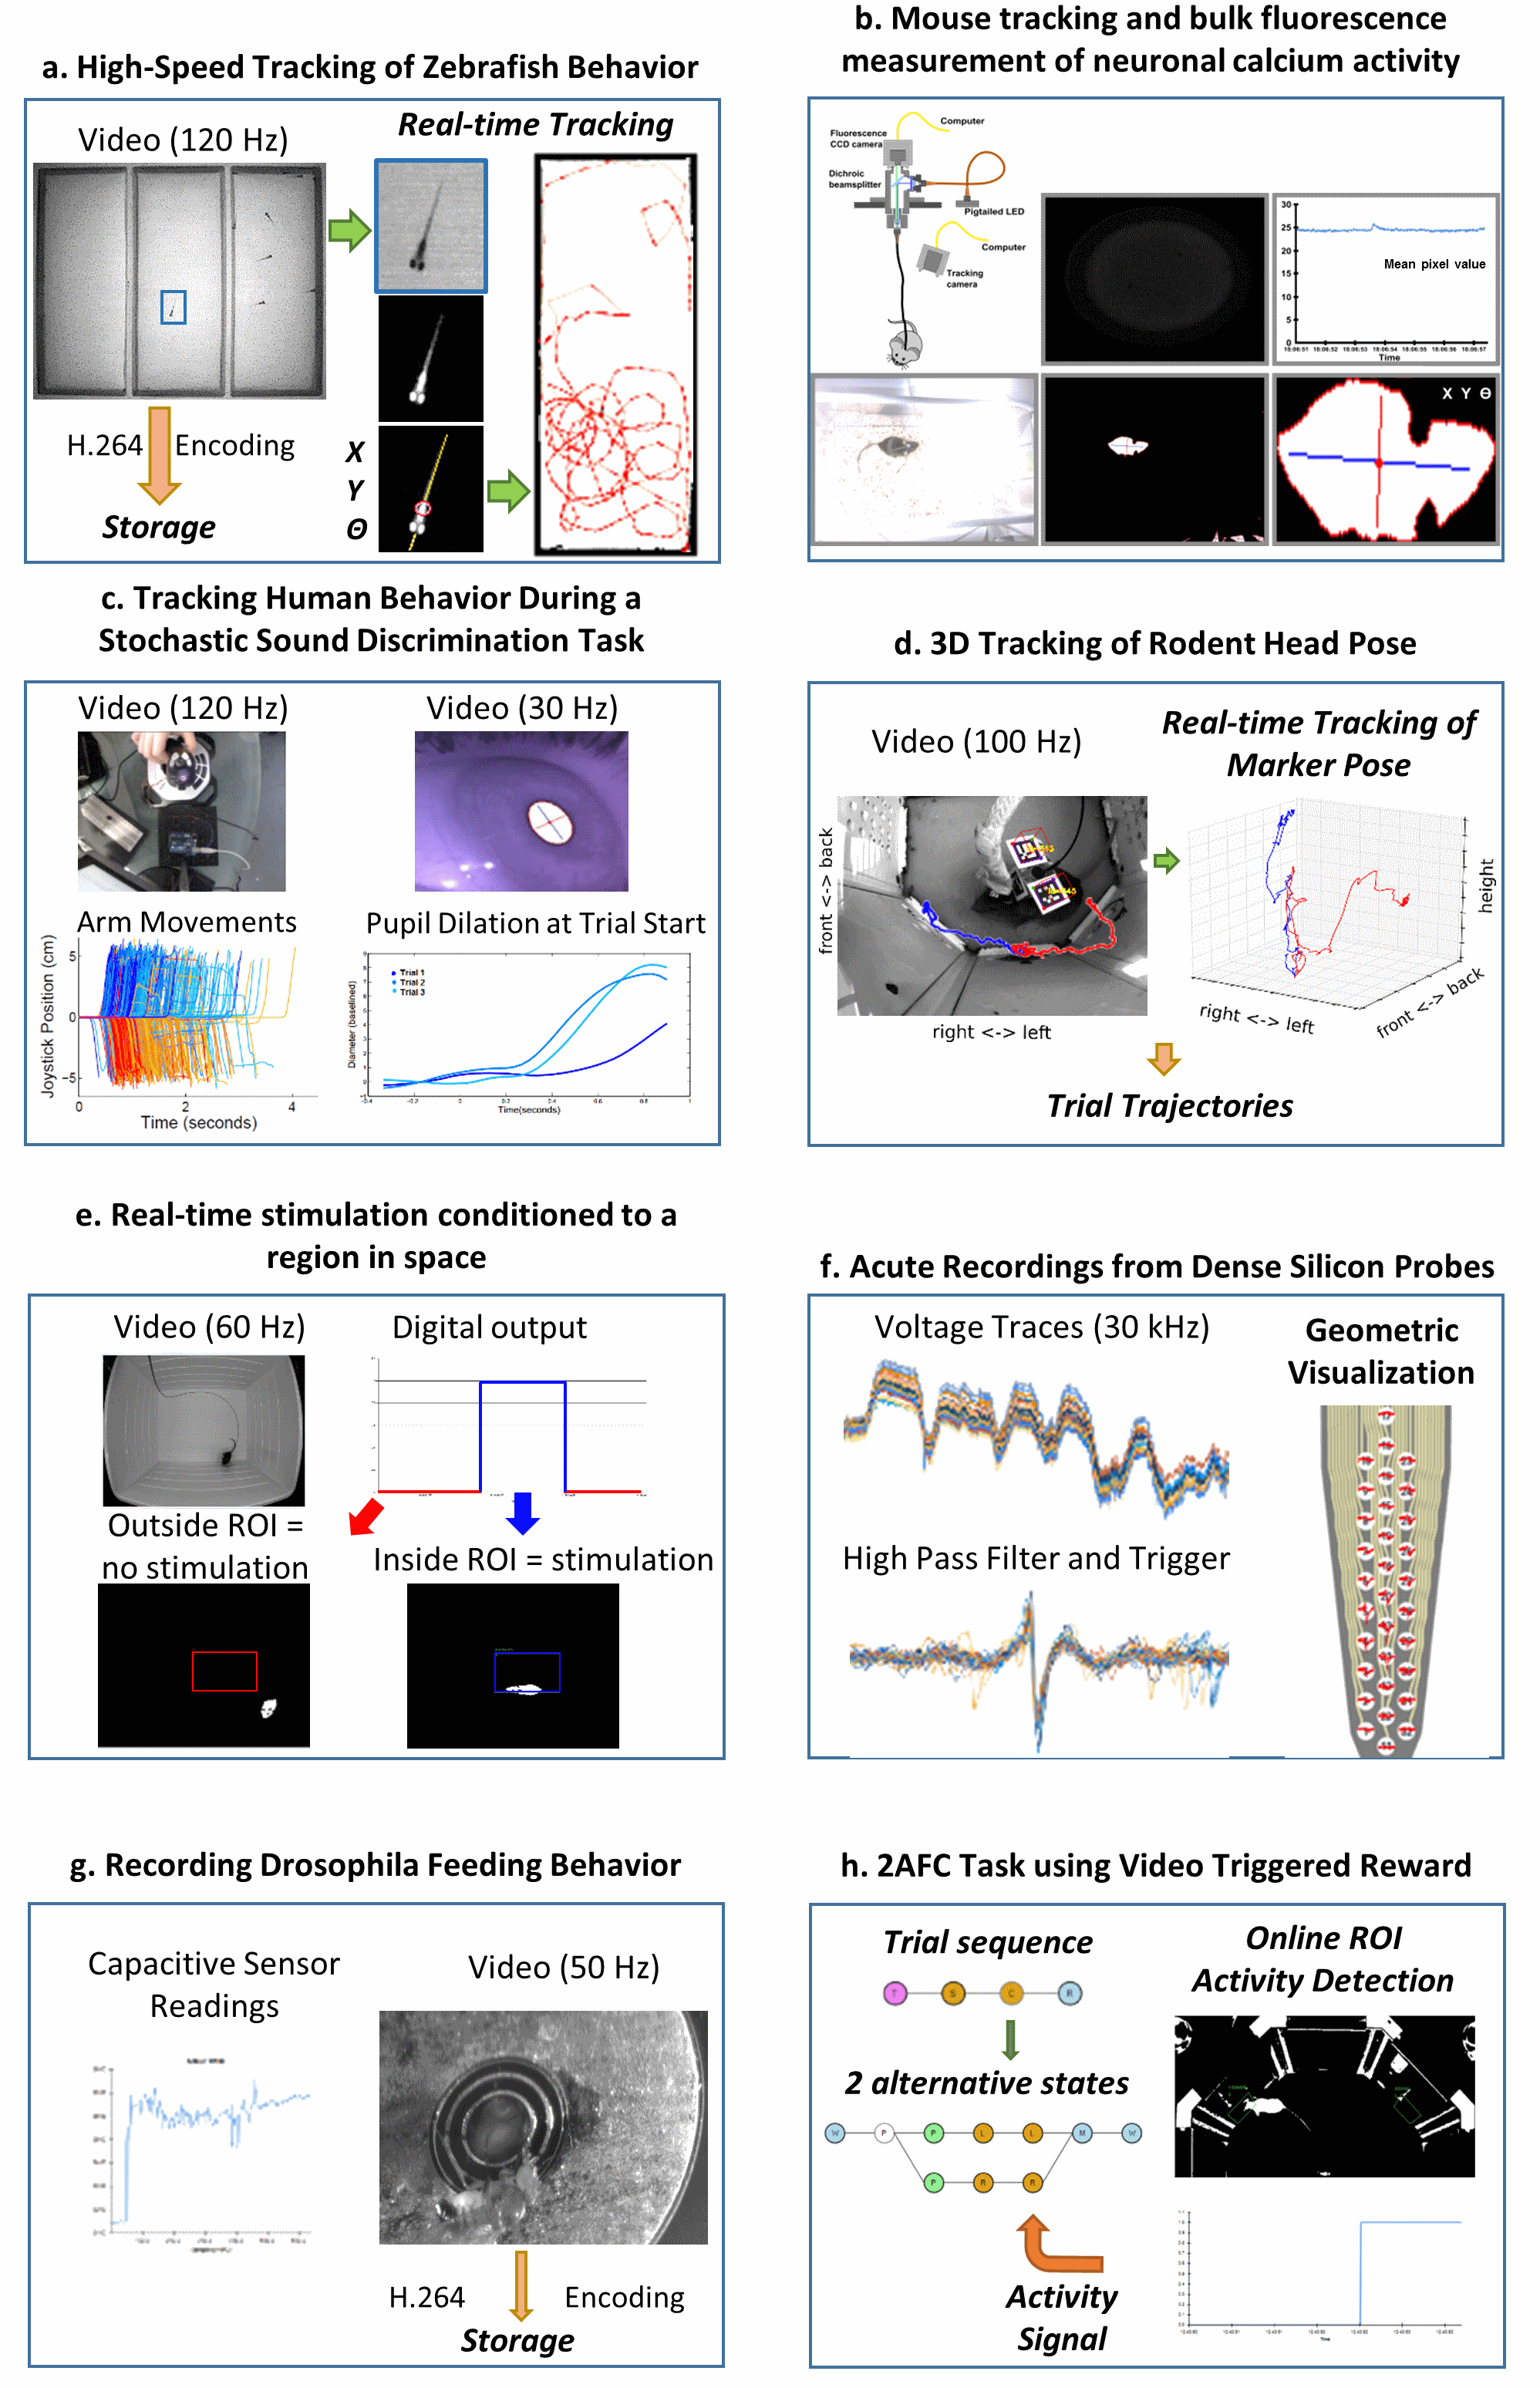
\includegraphics[width=\linewidth]{chapters/figuresChTools/bonsaiApplications.png}}
\end{center}
\vspace{-5mm}
\caption{Example neuroscience experimental setups using Bonsai.}
\label{fig:bonsaiApplications}
\end{figure}

One of the first use cases driving the development of Bonsai was the automated online tracking of animal behaviour using video. The most common tracking application involves chaining together operators for image segmentation and binary region analysis to allow the extraction of the spatial location of an animal over time (Figures \ref{fig:bonsaiApplications}A,B). The same technique can easily be extended to track different kinds of objects, such as eyes or experimental manipulanda in human psychophysics experiments (Figure \ref{fig:bonsaiApplications}C), provided adequate illumination contrast and the appropriate choice of a method for segmentation. These image processing tools can also be used to acquire and process physiological data in neural imaging setups, where it is now possible to record bioluminescent or fluorescent reporters of neural activity during behaviour. For example, Figure \ref{fig:bonsaiApplications}B demonstrates simultaneous measurement of animal behaviour and neural activity using bulk fluorescence calcium imaging in the mouse brain recorded with a CCD sensor and a fiberoptic system \cite{Tecuapetla2014}.

Raw video data from modern high-resolution, high-speed cameras can be expensive and cumbersome to store. Online video compression and storage sinks were implemented taking advantage of parallelism to avoid frame loss. Video compression is processing intensive and can compromise data acquisition if reading the next frame has to wait for the previous frame to be fully encoded. One solution is to buffer incoming frames and compress them in parallel with the rest of the processing stream. By encapsulating this behaviour into a Bonsai sink, it became easy to incorporate video recording and compression functionality into any image processing pipeline (Figures \ref{fig:bonsaiApplications}A–E,G,H).

While simple image processing techniques can easily extract continuous two-dimensional measures of animal location over time, it often becomes the case that the experimenter is concerned with tracking the detailed behaviour of specific features in the animal's body, such as head pose. This is an essential component in neurophysiology or stimulation experiments in freely moving animals, where ongoing behaviour is the central constraint in interpreting neural responses and manipulations. However, identifying such features and reconstructing their position and orientation in 3D space is a challenging computer vision problem. A common solution is to use planar fiducial markers of known geometry \cite{Kato1999, Garrido-Jurado2014} (Figure \ref{fig:bonsaiApplications}D). The computer vision research community has developed some open-source software solutions to this problem \cite{Garrido-Jurado2014}, which have been integrated into Bonsai to allow the possibility of easily and flexibly incorporating online 3D fiducial tracking in video streams. This approach has been used successfully to record 3D head movements of a mouse under optogenetic stimulation in a decision-making task (Figure \ref{fig:bonsaiApplications}D).

One final, but important application of video stream processing is in the development of closed-loop interfaces, where the actions of an animal directly modulate manipulations under the experimenter's control. This kind of experiment requires fast online analysis of behaviour and physiological variables of interest that are subsequently coupled to hardware control interfaces. In Figure \ref{fig:bonsaiApplications}E, real-time stimulation conditioned to a region in space was implemented by analyzing the position of an animal in a square arena. Whenever the animal found itself inside a specified region of interest, a signal was sent to an Arduino controller which was then used to drive optogenetic stimulation of specific neural circuits.

Another key data type that is commonly processed by Bonsai dataflows is buffered time-series data. This type of data usually arises from audio, electrophysiology or other digital acquisition systems where multiple data samples, from one or more channels, are synchronously acquired, buffered and streamed to the computer. These buffers are often represented as data matrices, where rows are channels and columns represent individual data samples through time, or vice-versa. Support for simple band-pass filters, thresholding and triggering allowed us to build flexible spike detection and waveform extraction systems (Figure \ref{fig:bonsaiApplications}F). Using Intan's Rhythm API, we integrated into Bonsai support for a variety of next-generation electrophysiology devices using Intan's digital amplifier technology, such as the Open Ephys acquisition system \cite{Voigts2013} or Intan's evaluation board (RHD2000, Intan Technologies, US). This system was successfully used to acquire and visualize simultaneous recordings from dense silicon probes where spikes from a loose-patch juxtacellular pipette were used as triggers to align and extract waveform data appearing on the multi-channel extracellular probe. Responses from every silicon probe site could then be superimposed on an accurate rendition of the probe geometry, in real-time.

The ability to rapidly integrate new modules allowed us to support the development and cross-validation of new tools for behavioral neuroscience. A paradigmatic example was the flyPAD, a new method for quantifying feeding behaviour in Drosophila melanogaster by measuring changes in electrode capacitance induced by the proboscis extension of a fly \cite{Itskov2014}. The integration of the flyPAD in Bonsai allowed researchers to quickly get started using this approach to design new experiments. Furthermore, it also allowed the validation of the tool by enabling simultaneous acquisition of high-speed video recordings of fly behaviour which were later used for annotation and classification of the sensor feeding traces (Figure \ref{fig:bonsaiApplications}G).

In a different set of experiments, Bonsai was used to implement a variation on a popular two-alternative forced choice (2AFC) decision-making task for rodents (Figure \ref{fig:bonsaiApplications}H). In this type of task, animals are placed in an environment with three “ports.” They are presented with a stimulus in the center port and afterwards report their perception of the stimulus by going either to the left or right choice ports. In the variation we present in this work, the two choice ports were replaced by regions of interest where the activity of the animal is analyzed using computer vision. This example offered unique challenges as it combined sophisticated sequential control of a task environment with continuous data stream processing of video and sensor data.

The integration of all these diverse components for data acquisition and experiment control does not only allow for the rapid deployment of established protocols. In fact, the modular nature of their integration (i.e., how they can be combined together) opens up new avenues for research, by allowing a rich, rapid exploration of novel methodologies. To demonstrate this, we created a dynamic virtual environment for freely moving rodents where the visual presentation of a stimulus is tightly controlled in closed-loop to the actions of the animal. We used a projection setup similar to the low-cost multi-touch sensing table proposed by \cite{Han2005}, where a visible light rear-projection system is coupled with infrared illumination and an infrared imaging sensor to detect in real-time where the animal is located with respect to the visual display surface (Supplementary Video 2).
